\chapter{Divide-and-Conquer Lexer}
An incremental divide and conquer lexer works by dividing the sequence, to be lexicaly analysed,
into small parts and analyse them; and then combining them. In the base
case the lexical analysis is done on a single character. The conquer step
then combines the smaller tokens into as large tokens as possible. The end
result is a sequence of token that represent the code. How this is done
will be described below.

\section{Divide and Conquer in General}
This section gives an idea of how the Divide and Conquer algorithm
works in general, before adressing in detail how to apply it to lexing.
% So when talking about the incremental lexer there is an understanding about the underlying techniques.

\subsection{The Three Steps}
The general idea of a divide and conquer algorithm is to divide a problem into
smaller parts and solve them separatly and then combine the results. A Divide
and Conquer algorithm always consists of a pattern with these three steps \cite{Goodrich}.
\begin{description}
\item[Divide:] If the input size is bigger than the base case then divide the
input into subproblems. Otherwise solve the problem using a straightforward
method.
\item[Recur:] Recursively solve the subproblems associated with the subset.
\item[Conquer:] Given the solutions to the subproblems, combine the results to
solve the original problem.
\end{description}

\subsection{Associative Function}
An associative function, or operator, is a function that doesn't care in what
order it is applied. An example of such a function is $+$, which is associative
since it has the propert in \cref{assprop}.

In divide and conquer algorithms this is essential. In the divide step of the
divide and conquer algorithm, there is no certain order of how the subproblems
are going to be divided. This means that the order the subproblems are being
conquered can't have an impact on the algorithm, hence the conquer step must be
associative.

\begin{example}[Associativity of the conquer step]\label{assprop}
Let $f(x,y)$ be the conquer function, where $x$ and $y$ are of the same type as
the result of $f$, then:
\begin{center}
$f(x,f(y,z)) \to a$\\
$f(f(x,y),z) \to b$\\
$a=b$
\end{center}
Otherwise the algorithm can give different results for the same data.
\end{example}

\subsection{Time Complexity}
To calculate the running time of any divide and conquer algorithm the master
method can be applied \cite{Cormen}. This method is based on the following
theorem.
\begin{theorem}[Master Theorem \cite{Cormen} \label{MasterTheo}] $ $\\
Assume a function $T_n$ constrained by the recurrence
\begin{center}
$T_n = {\alpha}T_{\frac{n}{\beta}}+ f(n)$
\end{center}
(This is typically the equation for the running time of a divide and conquer algorithm, where $\alpha$
is the number of sub-problems at each recursive step, $n/\beta$ is the size of
each sub-problem, and $f(n)$ is the running time of dividing up the problem
space into $\alpha$ parts, and combining the sub-results together.)\\
If we let $e = log_\beta \alpha$, then
\begin{center}
\begin{tabular}{r c l l}
1. $Tn$ & $=$ & $\Theta(n^{e})$ &  if $f(n) = O(n^{e - \epsilon})$ and $\epsilon > 0$\\
2. $Tn$ & $=$ & $\Theta(n^{e} log n)$ & if $f(n) = \Theta(n^e)$\\
3. $Tn$ & $=$ & $\Theta(f(n))$ & \begin{minipage}[t]{0.6 \columnwidth}
  if $f(n) = \Omega(n^{e+\epsilon})$ and $\epsilon > 0$
  and $\alpha \cdot f(n/\beta) \leq c \cdot f(n)$
  where $c < 1$ and all sufficiently large $n$
  \end{minipage}
\end{tabular}
\end{center}
\qeda
\end{theorem}

\subsection{Hands on Example}
The divide and conquer pattern can be preformed on different sorts of algorithm
that solves different problems. A general problem is sorting, or more precisely
sorting a sequence of integers. This example shows merge-sort.

\begin{description}
\item[divide:] The algorthim starts with the divide step. Given the input $S$ the algorithm
will check if the length of $S$ is less then or equal to 1.
\begin{itemize}
\item If this is true, the sequence is returned. A sequence of one or zero
elements is always sorted.
\item If this is false, the sequence is split into two equaly big sequences,
$S_1$ and $S_2$. $S_1$ will be the first half of $S$ while $S_2$ will be the
second half.
\end{itemize}
\item[Recur:] The next step is to sort the subsequences $S_1$ and $S_2$. The sorting
function sorts the subsequences by recursivly calling itself twice with $S_1$ and
$S_2$ as arguments respectivly.
\item[Conquer:] Since $S_1$ and $S_2$ are sorted combining them into one sorted
sequence is trivial. This process is what's refered to as merge in merge-sort.
The resulting sequence of this merge is returned.
\end{description}
Algortihm~\ref{Alg:MergSort} shows a more formal definition of merge-sort.

\begin{algorithm}
\DontPrintSemicolon
\KwData{Sequence of integers $S$ containing $n$ integers}
\KwResult{Sorted sequence $S$}
\If {$length(S) \leq 1$}{
  \Return $S$ \;
}
\Else {
  $(S_1,S_2) \gets splitAt(S,n/2)$ \;
  $S_1 \gets MergeSort(S_1)$\;
  $S_2 \gets MergeSort(S_2)$\;
  $S \gets Merge(S_1, S_2)$\;
  \Return $S$
}
\caption{MergeSort}
\label{Alg:MergSort}
\end{algorithm}

Given the mergesort algorithm, time complexity can be calculated as follows
using the master method. There are $2$ recursive calls and the subproblems are
$1/2$ of the original problem size, so $\alpha=2$ and $\beta=2$. To merge the two sorted subproblems the
worst case is to check every element in the two list, $f(n) = 2 \cdot n/2 = n$.
\begin{center}
 $T(n) = 2T(n/2) + n$.
\end{center}
Results in: 
\begin{center}
$a = 2$, $b = 2$ and $f(n) = n \;
\Rightarrow n^{log_b a} = n^{log_2 2} = n$
\end{center}
Case 2 of the master theorem applies, since
\begin{center}
$f(n) = O(n)$
\end{center}
So the solution will be:
\begin{center}
$T(n) = \Theta(n^{log_2 2} \cdot log n) = \Theta(n \cdot log n)$
\end{center}

\section{Divide and Conquer Lexing in General}
In the last section we covered the general divide and conquer algorithm. In this
section the general data structures and algorithms for an incremental divide and
conquer lexer are covered.

\subsection{Treestructure} % work in progress.
The incremental divide and conquer lexer should use a structuer where the
code-lexemes can be related to its tokens, current result can be saved and easy
recalculated. A divide and conquer lexer should therefore use a tree structure
to save the lexed result in. Since every problem can be divided in to several
subproblems, until the basecase is reached. This is cleraly a tree structure of
solutions, where a leaf is a token for a single character. and the root
is a sequence of all tokens in the code.  

%TODO master thereom

\subsection{Transition map} % before treestructure?
When storing a result of a lexed string it is a good idea to store more then
just the tokens. In particular the in and out states are needed when combining
the lexed string with another string. We will henceforth refer to this as a
$transition$.
\begin{verbatim}
type Transition = (State,[Token],State)
\end{verbatim}
Since the lexer doesn't know if the current string is a prefix of the entire
code or not it can't make any assumptions on the in state. Because of this the
lexer needs to store a transition for every possible in state, we will henceforth
refer to this as a \emph{transition map}.
\begin{verbatim}
type Transition_map = [Transition]
\end{verbatim}
\subsection{The Base Case}
When the lexer tries to lex one character it will create a transition
map using the DFA for the language. It will for each state create a transition
that has the state as in state, a list containing the character as the only
token and by using the DFA, lookup what out state the transition should have.
For the character '/' part of a transition map might look like the following.

In the
examples below the first number refers to the in state, the middle part is the
sequence of tokens and the second number is the out state, that can be accepting.
\begin{center}
$\left[\begin{array}{ccc}
10&Single '/'&10\\
11&Single '/'&NoState\\
12&Single '/'&10\\
\end{array}\right]$
\end{center}
$NoState$ transition is used to tell the lexer that using that particular 
transition will result in a lexical error. For reasons being covered in
\cref{longmatch}, they can't be discarded.

\subsection{Conquer Step}
The conquer step of the algorithm is to combine two transition maps in to one
transition map. This is done by, for every transtion in the left transition map, combining
the transition with the transition in the right transition map that has the same in state as the
left transitions out state.

The most general case is a naive lexer that takes the first accepting state it
can find. When two transition maps are combined there are two different outcomes:
\begin{description} 
  \item[Concat:]If the out state of the first transition is accepting, the
    sequence in the transition that starts in the starting state of the second
    transition map will be appended to the first.\\
\#Look over syntax in this example
\begin{center}
$NewTOKENS=TOKENS1 >< TOKENS2$
\end{center}
%create two tokens if the
%    out state of the first list is accepting then the second list will be appended
%    to the first list.
  \item[Combine:]If the out state of the first transition is not accepting, the
    transition in the second transition map with the same in state as the out
    state of the first transition will be used. The last token of the sequence
    from the first transition will be combined with the first token in the second
    transition in to one token and put between the two sequences.\\
\#Look over syntax in this example
\begin{center}
$TOKENS1=PREFIX1|>token1$\\
$TOKENS2=token2<|SUFFIX2$\\
$newtoken=token1 `combinedWith` token2$\\
$NewTOKENS=PREFIX1 |> newtoken >< SUFFIX2$\\
\end{center}
%The other case is when the first list of tokens does not end
%    in an accepting state. In this case the lexer will try to find an in state in
%    the second list that is the same as the out state of the first transition.
\end{description}
For both the cases the in state of the first transition will be the new in state
and the out state of the second transition will be the new out state.
\begin{center}
$\left[\begin{array}{ccc}
0&Single '/'&1\\
1&Single '/'&Accepting 5\\
\end{array}\right] `combineTokens`
\left[\begin{array}{ccc}
0&Single '/'&1\\
1&Single '/'&Accepting 5\\
\end{array}\right] =
\left[\begin{array}{ccc}
0&Single '//'&Accepting 5\\
1&Multiple '/' [] '/'&Accepting 1\\
\end{array}\right]$
\end{center}
This won't work as a lexer for most languages since it will lex a variable to
variables where the length is a single character, for example ``os'' will be
lexed as two tokens, ``o'' and ``s''. To solve this some more work is needed to
be done.

\subsection{Longest Match}\label{longmatch}
Instead of taking the naive aproach where a token is created if the lexer finds an
accepting state, the rule for creating a new token will instead be when the
combination of two transitions yields $NoState$ the lists will be appended. That
is, when there is an out state from the first transition that corresponds to an
in state of the second transition and the out state of the second transition
isn't $NoState$, the last token of the first transition and the first token of
the second transition will become one token, otherwise append the second list to
the first list.
%When two list of tokens are combined there are two cases that can emerge. The
%first being that a transition from the first list has an out state that
%corresponds to an in state with a valid out state, i.e. not $NoState$, in the
%second list of transitions. In this case the sufix of the first transition will
%be paired with the prefix of the second and seen as a complete token.
\begin{center}
$\left[\begin{array}{ccc}
0&Single '//'& Accepting 5\\
1&Multiple '/' [] '/' &1\\
\end{array}\right] `combineTokens` 
\left[\begin{array}{ccc}
0&Single '\textbackslash n'&Accepting 6\\
1&Single '\textbackslash n'&1\\
5&Single '\textbackslash n'&NoState\\
\end{array}\right] =
\left[\begin{array}{ccc}
0&Multiple '//' [] '\textbackslash n'&Accepting 6\\
1&Multiple '/' [] '/\textbackslash n'&1\\
\end{array}\right]$
\end{center}
The second case is when the out state for the right token list is $NoState$.
This means that the two lists of tokens can't be combined. In this case the
first token in the second list will be viewed as the start of a token and the
last token in the first list will be viewed as the end of a token.

\begin{figure}[!htp]
\centering
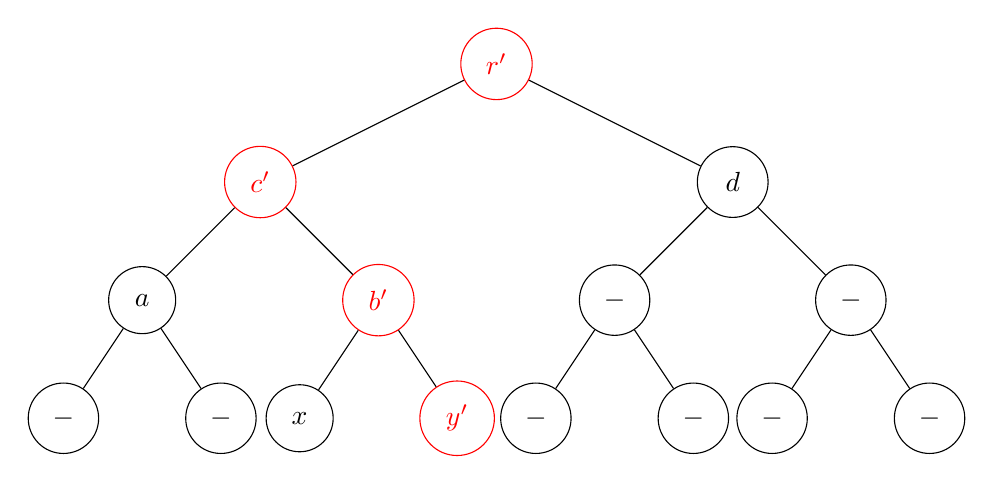
\begin{tikzpicture}[level/.style={sibling distance=60mm/#1, align=center, text centered}]
\node [circle,red,draw, text width = 1.5em, text centered] (z){$r'$}
  child {node [circle,red,draw, text width = 1.5em] (a) {$c'$}
    child {node [circle,draw, text width = 1.5em] (b) {$a$}
      child {node [circle,draw, text width = 1.5em] (c) {$-$}} 
      child {node [circle,draw, text width = 1.5em] (d) {$-$}}
    }
    child {node [circle,red,draw, text width = 1.5em] (e) {$b'$}
      child {node [circle,draw, text width = 1.5em] (f) {$x$}}
      child {node [circle,red,draw, text width = 1.5em] (g) {$y'$}}
    }
  }
  child {node [circle,draw, text width = 1.5em] (i) {$d$}
    child {node [circle,draw, text width = 1.5em] (j) {$-$}
      child {node [circle,draw, text width = 1.5em] (k) {$-$}}
      child {node [circle,draw, text width = 1.5em] (l) {$-$}}
    }
    child {node [circle,draw, text width = 1.5em] (m) {$-$}
      child {node [circle,draw, text width = 1.5em] (n) {$-$}}
      child {node [circle,draw, text width = 1.5em] (o) {$-$}}
    }
  };
\end{tikzpicture}
\caption{Incremental Computing, the updated nodes when a leaf changes \label{fig:incUp}}
\end{figure}

\subsection{Incremental Computing}
To be incremental means that, whenever some part of the data to the algorithm
changes the algorithm tries to save time by only recomputing the changed data
and the parts that depend on this changed data. \cite{incrementalDef}

For a divide and conquer lexer this would mean only recompute the changed token and the token to the right of the changed token. This is done recurrsivly until the root of the tree is reached. The expected result of this would be that when a character is added to the code of 1024 tokens, instead of relex all 1024 tokens the lexer will only do 10 recalculations for new tokens. Since, $log_2 1024 = 10$. This can be explained by the \cref{MasterTheo}. How this is calculated for an incremental divide and conquer lexer is described more in detail in the next sub-section.

\subsection{Expected Time Complexity}
Since incremental computing stated that only content which depends on the new data will be recalculated. That is, follow the branch of the tree from the new leaf to the root and recalculated every node on this path. 
As shown by \cref{fig:incUp}. Only one subproblem is updated in every level of the tree. Back to the master theorem. Let put this in to numbers, $e = log_b a$ where $a$ is number of recursive calls and $n/b$ is size of the subproblem where $n$ is the size of the original problem. As shown by the \cref{fig:incUp} number of needed update calls is $1$, therefor $a = 1$. The constant $b$ is still $2$. This will give $e = log_2 1 = 0$. Thus the update function of the incremental algorithm will have a time complexity of $\Theta(n^0 \cdot log n) = \Theta(log n)$

\section{Pitfalls}
This section will describe techniques that were tried under the constuction of 
the incremental divide and conquer lexer but was shown to give bad results.

\subsection{Brutefore}
The first naive solution was to "bruteforce" to find the lex. This was showned to be to resource-eating. But it describes the general idea of how the problem could be solved. Why it was a bad solution will be described futher on in the text. 

The above rules will work for very simple languages. When comments are
introduced you will get the problem that the whole code can be one long partial
comment token. To remedy this you can add two rules:
\begin{itemize}
\item Every time you combine two tokens you only do so if the combination has a
transition from the starting state.
\item If two tokens can be combined completly, check if the next token can be
combined aswell.
\end{itemize}
This ensures that every token starts in the starting state and that each token
is as long as it can be.

This also has some problems though. When keywords like ``else if'' are
introduced the lexer will start to lex like in \cref{elseif}. To solve this the
lexer checks when two tokens are completely uncombinable if the first of these
have an accepting state as outgoing state. If the token don't have an accepting
out state, the lexer tries to break up the token until it does. The exception to
this rule is single characters which are permitted to not have no accepting out
states.
\begin{example}[else if lexing]\label{elseif}
Somewhere in the middle of the code ``... 1 else 0 ...''
\begin{center}
\begin{tabular}{ll}
String & Type\\
1 & $Number$\\
\_ & $Space$\\
else\_ & $Nothing$\\
0 & $Number$\\
\end{tabular}
\end{center}
\end{example}

\begin{example}[Devide and Append]
The lexer will always try to build as lage tokens as possible. When it realizes that this cant be done it has to backup and try to combine the parts in a different way. This example will show how this is done in theory. 

The code segment for this example is: 
\begin{center}
"else return".
\end{center}
The tree in \cref{fig1:elseif} shows the first step of the token combine rutine. Clearly this returns a nonexsisting token. 
\begin{figure}[h!]
  \centering
  \begin{tikzpicture}[
    error/.style={rectangle, draw=none, rounded corners=1mm, fill=black!20!red, drop shadow,
        text centered, anchor=north, text=white},
    fact/.style={rectangle, draw=none, rounded corners=1mm, fill=black!60!green, drop shadow,
        text centered, anchor=north, text=white},
    state/.style={rectangle, draw=none, rounded corners=1mm, fill=blue, drop shadow,
        text centered, anchor=north, text=white},
    leaf/.style={rectangle, draw=none, rounded corners=1mm, fill=blue, drop shadow,
        text centered, anchor=north, text=white},
    level distance=0.5cm, growth parent anchor=south
    ]
    \node (State00) [error] {NoToken} [->]
        child{ [sibling distance=9cm]
            node (State01) [state] {"else return"}
            child{
                node (Fact02) [fact] {PossibleToken(ElseIf)}
                child{ [sibling distance=4cm]
                    node (State02) [state] {"else "}
                    child{
                        node (Fact03) [fact] {Token(Else)}
                        child{
                            node (State03) [leaf] {"else"}
                        }
                    }
                    child{
                        node (Fact04) [fact] {Token(WhiteSpace)}
                        child{ [sibling distance=1.2cm]
                            node (State04) [leaf] {" "}
                        }
                    }
                }
            }
            child{ [sibling distance=4cm]
                node (Fact05) [fact] {Token(Return)}
                child{
                    node (State05) [leaf] {"return"}
                }
            }
        }
    ;
  \end{tikzpicture}
  \caption{Lexer thinks "else " is an "else if" pattern. 
  \label{fig1:elseif}}
\end{figure}
From here when the lexer has found that there are no tokens for this lexeme it will try to split the left child token.
\begin{center}
    split("else ") => ["else"," "]
\end{center} 
Now the lexer has a pair of two lexems that represent valid tokens. The lexer knows that combinding these two lexems in the pair returns in a NoToken result. So The only thing to do is to try to combine the right token in the pair with the right child token and let the token to the left in the pair stand alone. 
\begin{figure}[!h]
  \centering
  \begin{tikzpicture}[
    error/.style={rectangle, draw=none, rounded corners=1mm, fill=black!20!red, drop shadow,
        text centered, anchor=north, text=white},
    fact/.style={rectangle, draw=none, rounded corners=1mm, fill=black!60!green, drop shadow,
        text centered, anchor=north, text=white},
    state/.style={rectangle, draw=none, rounded corners=1mm, fill=blue, drop shadow,
        text centered, anchor=north, text=white},
    leaf/.style={rectangle, draw=none, rounded corners=1mm, fill=blue, drop shadow,
        text centered, anchor=north, text=white},
    level distance=0.5cm, growth parent anchor=south
    ]
    \node (State00) [error] {NoToken} [->]
        child{ [sibling distance=4cm]
            node (State01) [state] {" return"}
            child{ [sibling distance=4cm]
                node (State02) [fact] {Token(WhiteSpace)}
                child{
                    node (Fact02) [leaf] {" "}
                }
            }
            child{ [sibling distance=4cm]
                node (Fact03) [fact] {Token(Return)}
                child{
                    node (State03) [leaf] {"return"}
                }
            }
        }
    ;
  \end{tikzpicture}
  \caption{Lexer tries to combine an white space with a return statement
  \label{fig4:elseif}}
\end{figure}
This also return a NoToken. So the same thing will be done again. The lexer tries to split the left child before NoToken was given. In this case the whitespace. 
\begin{center}
split(" ") => []
\end{center}
But becouse the whitespace is of the lowest form and is not build up by smaller tokens the resulting list from the split function will be empty. Now the lexer knows that this token must be by it self. The "return" is the last lexeme in this example code so the lexer can't combine it futher. Thus the lexer has found the resulting sequence of tokens:
\begin{center}
    [(Token(Else), "else"), (Token(WhiteSpace)," "), (Token(Return), "return")]
\end{center} 
\end{example}

\subsection{Dont know what to call this!}
When the code is divided the lexer doesn't know if the string (or character) it
lexes is the first, last or is somewhere in the middle of a token. Instead of
checking what type of token the string will be (if it were to begin from the
starting state) it saves all the possible state transitions for that string.

In the examples that follow below state 0 is considered the starting state and
state $1-6$ are considered accepting.
\begin{example}[Transition map for a token]\label{transMap}
A hypothetical transition map for the char 'i'.
\begin{center}$\begin{array}{cc}
\multicolumn{2}{c}{'i'}\\
in & out\\
0 & 1\\
1 & 1\\
8 & 7\\
\end{array}$\\
\end{center}
\end{example}
In the base case the lexer will map all the transitions for all individual
characters in the code and construct partial tokens of them. The conquer step
will then combine two of these at a time by checking which possible outgoing
states from the first token can be matched with incoming states from the second
token. If there are such pairs of outgoing states with incomming states, then a
new partial token is created.
\begin{example}[Combining two tokens]\label{combTok}
'if' can be an ident (state 1) or part of 'else if' (state 5).
\begin{center}$\begin{array}{cc}
\multicolumn{2}{c}{'i'}\\
in & out\\
\textcolor{brown}{0} & \textcolor{brown}{1}\\
1 & 1\\
\textcolor{blue}{8} & \textcolor{blue}{7}\\
\end{array}
`combineToken`
\begin{array}{cc}\multicolumn{2}{c}{'f'}\\
in & out\\
0 & 1\\
\textcolor{brown}{1} & \textcolor{brown}{1}\\
\textcolor{blue}{7} & \textcolor{blue}{5}\\
\end{array}
=
\begin{array}{cc}\multicolumn{2}{c}{'if'}\\
in & out\\
\textcolor{brown}{0} & \textcolor{brown}{1}\\
\textcolor{blue}{8} & \textcolor{blue}{5}\\
\end{array}$\\
\end{center}
\end{example}
If there are no pairs of outgoing states which match the incomming states the
lexer will try to combine the first token with as much of the second token as
possible. In this case there will be a remainder of the second token, The lexer
can now be sure that the begining of the remainder is the begining of a token
and that the merged part is the end of the token before.
Since the lexer knows the remainder is the begining of a token it strips all
transitions but the one that has incomming state as starting state. Since the
start token is the end of a Token it strips all but the transitions ending in an
accepting state.
\begin{example}[Combining a token a part of the second token]\label{combSplit}
'ie' ends in the accepting state for ident (1) and '\_' starts in the
starting state.
\begin{center}
$\begin{array}{cc}\multicolumn{2}{c}{'e\_'}\\
in & out\\
\textcolor{brown}{10} & \textcolor{brown}{8}\\
\end{array}
=
\begin{array}{cc}\multicolumn{2}{c}{'e'}\\
in & out\\
0 & 11\\
\textcolor{blue}{1} & \textcolor{blue}{1}\\
6 & 1\\
\textcolor{brown}{10} & \textcolor{brown}{9}\\
\end{array}
`combineToken`
\begin{array}{cc}\multicolumn{2}{c}{'\_'}\\
in & out\\
0 & 2\\
2 & 2\\
\textcolor{brown}{9} & \textcolor{brown}{8}\\
\end{array}
$\\
$\begin{array}{cc}
\multicolumn{2}{c}{'i'}\\
in & out\\
\textcolor{blue}{0} & \textcolor{blue}{1}\\
\textcolor{blue}{1} & \textcolor{blue}{1}\\
8 & 7\\
\end{array}
`combineToken`
\begin{array}{cc}\multicolumn{2}{c}{'e\_'}\\
in & out\\
10 & 8\\
\end{array}
=
\begin{array}{cc}\multicolumn{2}{c}{'ie'}\\
in & out\\
\textcolor{blue}{0} & \textcolor{blue}{1}\\
\textcolor{blue}{1} & \textcolor{blue}{1}\\
\end{array} ++ 
\begin{array}{cc}\multicolumn{2}{c}{'\_'}\\
in & out\\
0 & 2\\
\end{array}$\\
\end{center}
\end{example}
\# Perhaps remove this part\\
However the remainder may not have the start state as a possible incomming state.
In this case the lexer tries to find the largest possible token (that has the
starting state as incomming state) and tries to construct a token of the rest of
the remainder, repeating this procedure until the entire remainder has been
split into acceptable tokens. All the tokens accept the one that is on the very
end of the sequence will have all but their accepting states stripped. This case
does occur quite frequently since most languages has comments and strings which
can contain anything.
\begin{example}[Handling the remainder]\label{remToken}
'\_' starts in the starting states and ends in an accepting state and 'e' starts
in the starting state, it doesn't have to end in an accepting state.
\begin{center}
$\begin{array}{cc}\multicolumn{2}{c}{'\_i'}\\
in & out\\
\textcolor{brown}{9} & \textcolor{brown}{7}\\
\end{array}
=
\begin{array}{cc}\multicolumn{2}{c}{'\_'}\\
in & out\\
0 & 2\\
2 & 2\\
\textcolor{brown}{9} & \textcolor{brown}{8}\\
\end{array}
`combineToken`
\begin{array}{cc}
\multicolumn{2}{c}{'i'}\\
in & out\\
0 & 1\\
1 & 1\\
\textcolor{brown}{8} & \textcolor{brown}{7}\\
\end{array}$\\
$checkRemainder \left(\begin{array}{cc}\multicolumn{2}{c}{'\_i'}\\
in & out\\
9 & 7\\
\end{array} \right)
=
\begin{array}{cc}\multicolumn{2}{c}{'\_'}\\
in & out\\
0 & 2\\
\end{array} ++
\begin{array}{cc}\multicolumn{2}{c}{'i'}\\
in & out\\
0 & 1\\
\end{array}$\\
\end{center}
\end{example}
When all partial tokens has been combined in this way the resulting sequence of
tokens represents the the code the lexer was run on.

\section{Lexical Errors}
Since the lexer has to be able to handle any kind of possible not "complete"
tokens, error handling can be done in different ways. One approach is to simply
return as many tokens as possible from the code and where there might be lexical
errors the lexer returns the error in as small parts as possible.

\begin{example}[A lexer that only lexes letters] When the lexer encounters the
string "what @ day" it would return:
\begin{center}
\begin{tabular}{ll}
String & Type\\
What & $Word$\\
'\_' & $Space$\\
'@' & $No\_Token$\\
'\_' & $Space$\\
day & $Word$\\
\end{tabular}
\end{center}
\end{example}
